\documentclass[]{article}
\usepackage{amsmath}
	\numberwithin{equation}{section}
	\DeclareMathOperator{\arth}{arth}
\usepackage[colorlinks=true]{hyperref}
\usepackage[magyar]{babel}
\usepackage[T1]{fontenc}
\usepackage[utf8]{inputenc}
\usepackage{graphicx}
\usepackage{geometry}
\usepackage{anysize}
\usepackage{float}
\usepackage{physics}
\usepackage{slashed}
\marginsize{10mm}{10mm}{10mm}{10mm}
\newcommand\at[2]{\left.#1\right|_{#2}}


%opening
\title{Hálózati rendszerek és szolgáltatások fejlesztése}
\author{Lucienne Kachichian, Mikecz Kálmán, Németh Márton}

\begin{document}

\maketitle

\section{Docker használata}

\subsection{Docker telepítése}

\texttt{pacman -S docker}
\subsection{Docker image}

A fájlrendszer és a paraméterek összessége. Rétegekből épül fel, ezek az image létrehozása után csak olvashatóak.

\subsection{Docker container}
Amikor az image-et containerré alakítjuk (pl. \texttt{docker run}), akkor a docker egy írható/olvasható réteget helyez a csak olvasható rétegek felé.

\subsection{Dockerfile}

A dockerfile egy image leírását tartalmazza. Ez alapján a docker el tud készíteni egy image-et.

\section{Container vs VM}

	\textcolor{red}{IDE MÉG ÍRNI KÉNE}

\begin{figure}[H]
	\centering
	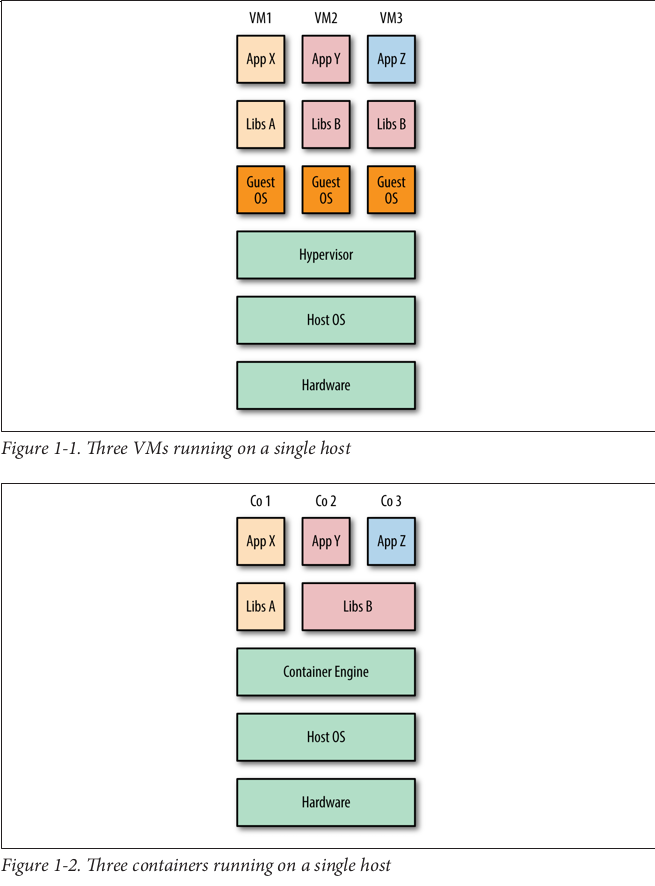
\includegraphics[width=0.9\linewidth]{cont_vs_vm}
	\caption{}
	\label{fig:contvsvm}
\end{figure}

\section{Példák docker futtatására}

\subsection{Hello World}

\texttt{docker run debian echo "Hello World"}

Ez a parancs futtatja a debian image-et, azon belül elindítja az echo programot, ami kiírja, hogy "Hello World".

\subsection{Két docker container kommunikációja}

Az első parancs elindítja a redis containert a háttérben, és elnevezi "myredis"-nek:

\texttt{docker run --name myredis -d redis}

A következő parancs elindít még egy redis containert. A link kapcsoló segítségével összekapcsolhatjuk a két containert, így a második container "redis" néven látja az elsőt. Ezt úgy éri el, hogy a \texttt{/etc/hosts} fájlba beírja az első, háttérben futó container IP-címét. A containerben elindul egy bash shell, itt a megfelelő parancsokat kiadva tudunk kommunikálni a másik containerrel.

\texttt{docker run --rm -it --link myredis:redis redis /bin/bash}

\begin{figure}[H]
	\centering
	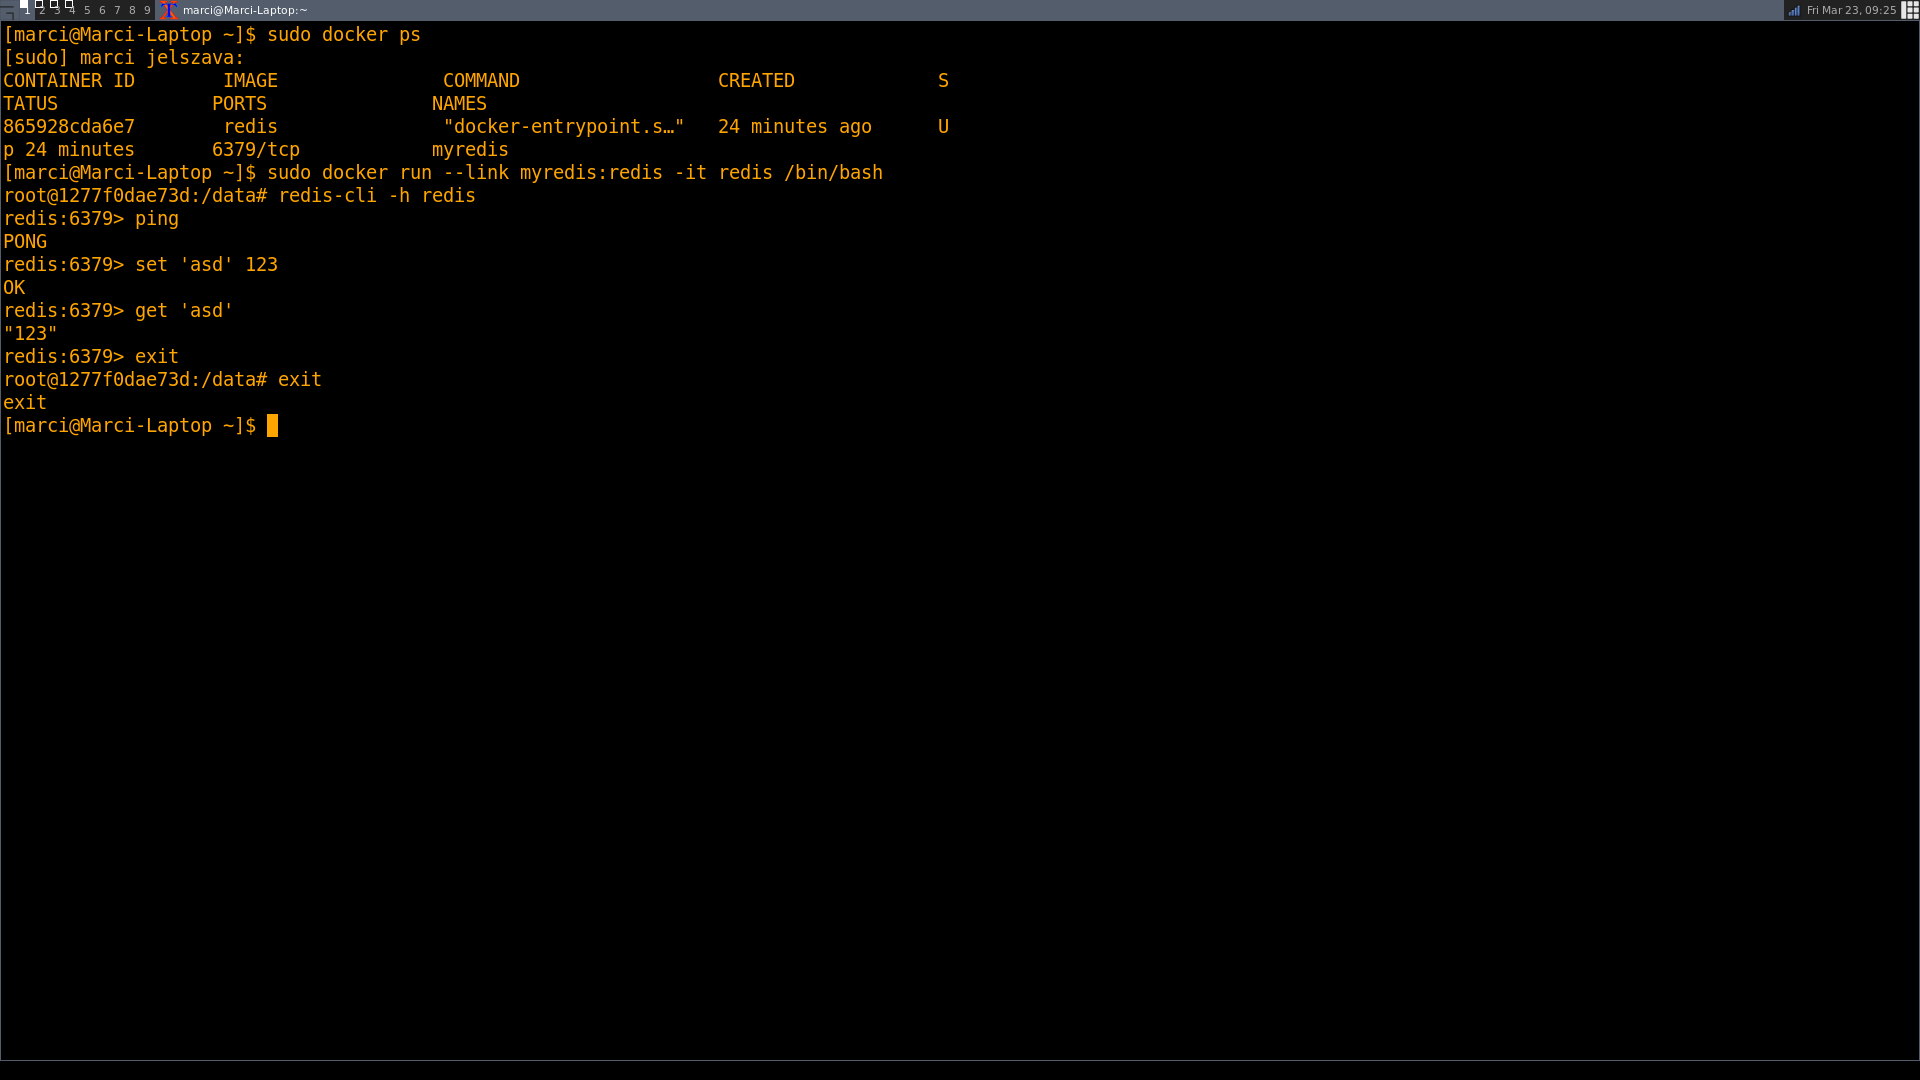
\includegraphics[width=0.9\linewidth]{redis.png}
	\caption{}
	\label{fig:redis}
\end{figure}

\section{Egyszerű docker webalkalmazás}

Az alábbi leírás alapján kipróbáltunk néhány egyszerű docker alkalmazást:

\texttt{https://github.com/docker/labs/blob/master/beginner/chapters/webapps.md}

\subsection{Statikus Nginx webalkalmazás}

Először egy statikus weboldalt jelenítettünk meg egy dockerben futó Nginx webszerver segítségével. Először letöltöttük és futtattuk a megfelelő docker image-et:

\texttt{docker run --name static-site -e AUTHOR="Your Name" -d -P dockersamples/static-site}

A \texttt{run} parancs letöltötte a \texttt{dockersamples/static-site} image-et, mert lokálisan nem találta meg. A kapcsolók szerepe:

\begin{itemize}
	\item \texttt{name}: megadja a container nevét, később így tudunk rá hivatkozni
	\item \texttt{e}: környezeti változókat állít be a containerber
	\item \texttt{d}: háttérben futtatja a containert
	\item \texttt{-P}: a container nyitott portjait a host egy-egy random portjára átirányítja
\end{itemize}

Ahhoz, hogy a host oldalról elérjük a weboldalt, tudnunk kell, hogy melyik porton érjük el a containert. Ezt az alábbi paranccsal kérdezhetjük le:

\texttt{docker port static-site}

Itt a \texttt{static-site} a container neve, amit korábban a \texttt{run} parancsnál megadtunk.

Ezután a webszervert elérhetjük a \texttt{localhost:port} címen, ahol a port helyére azt a portot kell írni, amit a \texttt{docker port} parancs megadott (a containeren belül a webszerver a 80-as porton fut). A webszerver működése a \ref{fig:webapp1}. ábrán látható.

\begin{figure}[H]
	\centering
	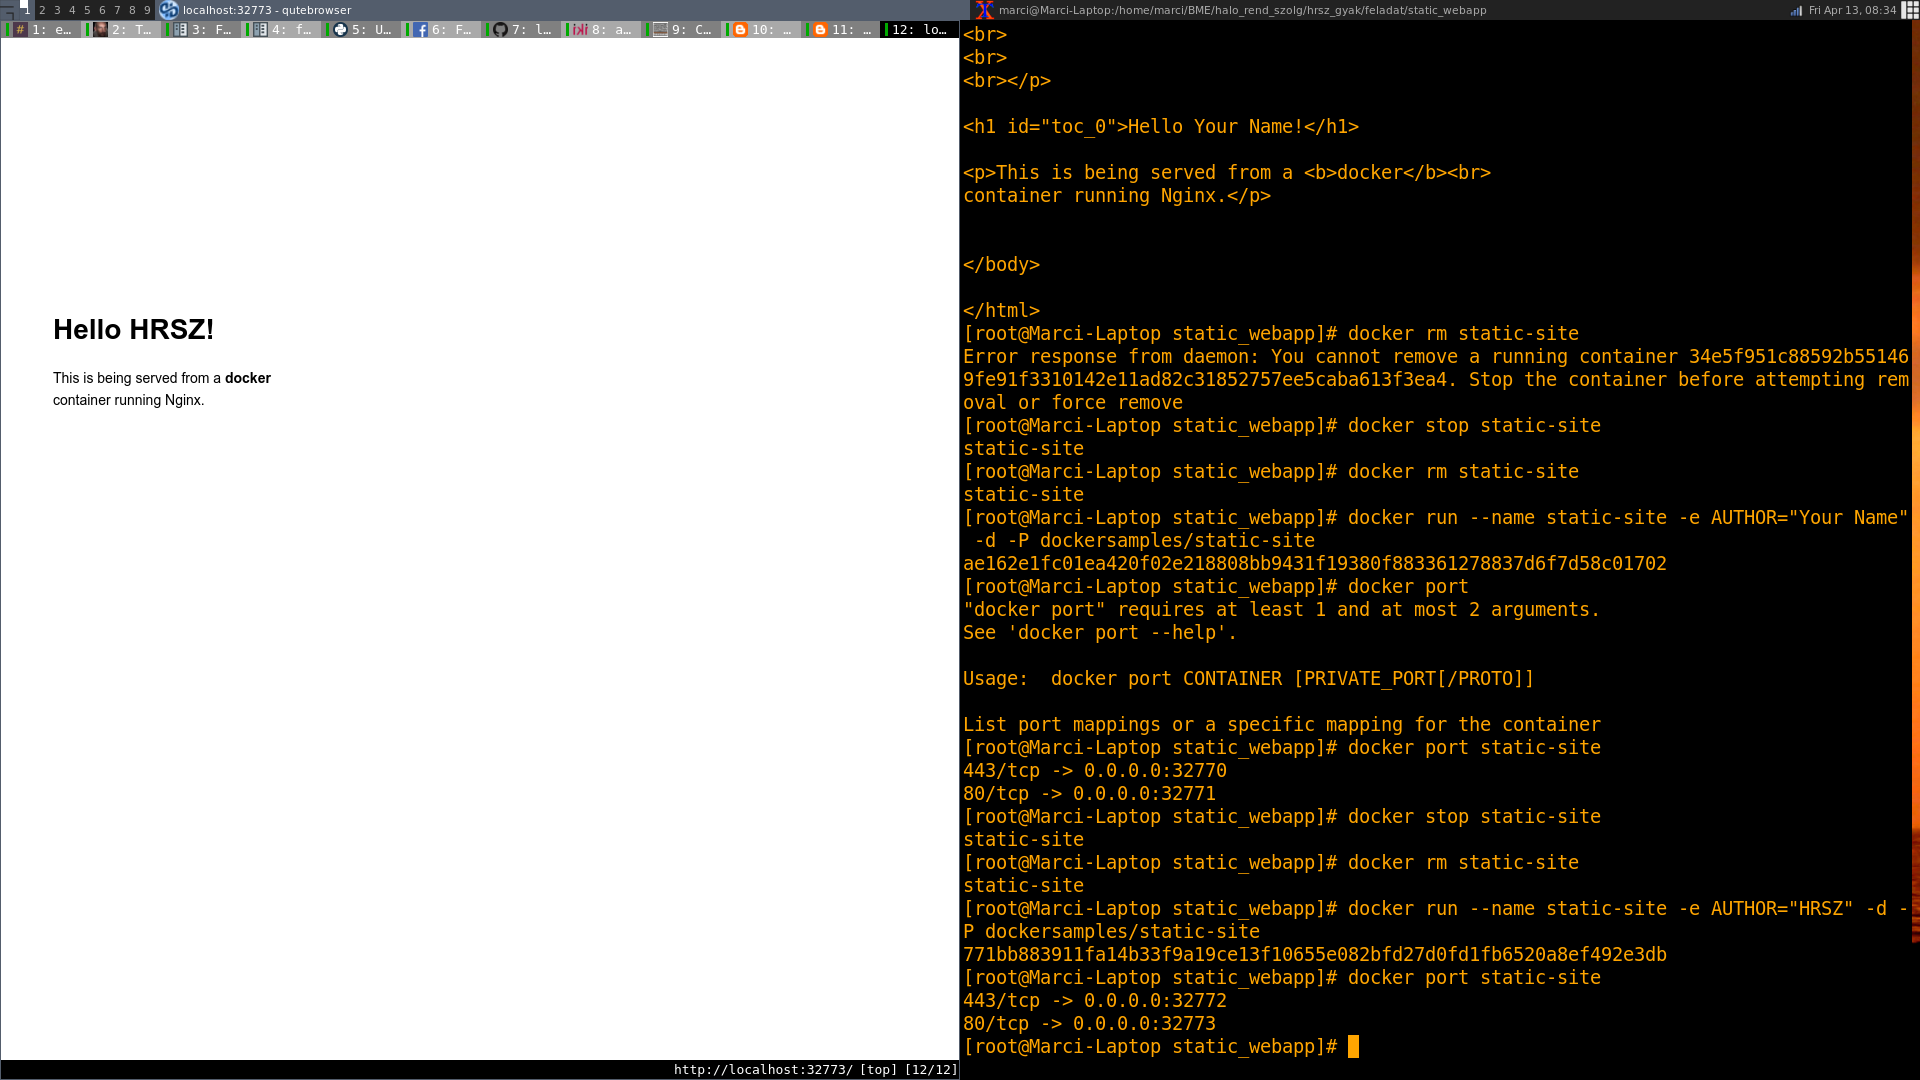
\includegraphics[width=0.9\linewidth]{webapp1}
	\caption{}
	\label{fig:webapp1}
\end{figure}

\subsection{Python Flask webalkalmazás létrehozása Dockerfile segítségével}

Az alábbi \texttt{Dockerfile} segítségével hoztuk létre a docker image-et:

\texttt{FROM alpine:3.5\\
	RUN apk add --update py-pip\\
	COPY requirements.txt /usr/src/app/\\
	RUN pip install --no-cache-dir -r /usr/src/app/requirements.txt\\
	COPY app.py /usr/src/app/\\
	COPY templates/index.html /usr/src/app/templates/\\
	EXPOSE 5000\\
	CMD ["python", "/usr/src/app/app.py"]}

A \texttt{Dockerfile} sorainak magyarázata:

\begin{itemize}
	\item \texttt{FROM alpine:3.5}: ezt a docker image-et használjuk kiindulásként. Az összes többi sor ehhez fog újabb rétegeket hozzáadni
	\item \texttt{COPY}: a hoston levő fájlt a docker image-be másolja a megadott helyre
	\item \texttt{RUN}: lefuttat egy parancsot a docker image build-elése közben
	\item \texttt{EXPOSE}: kinyitja a megadott portot
	\item \texttt{CMD}: megadja a container elindításakor lefuttatandó parancsot
\end{itemize}

A docker image által használt fájlok:

\begin{itemize}
	\item \texttt{requirements.txt}: ebben a fájlban van benne annak a python modulnak a neve, amit a \texttt{pip} csomagkezelővel fel kell telepíteni.
	\item \texttt{app.py}: ez maga a webszerver
	\item \texttt{templates/index.html} ez egy html template fájl, amit a webszerver felhasznál
\end{itemize}

Az alábbi paranccsal létrehozhatjuk az image-et:

\texttt{docker build -t alpine-flask .}

A \texttt{t} kapcsoló az image tag-et adja meg, később ezzel tudunk hivatkozni rá. A végén levő pont a \texttt{Dockerfile} helyét adja meg (jelen esetben az éppen aktuális könyvtár).

\vskip10pt
Ezután ugyanúgy futtathatjuk a containert, mint az előző példában:

\texttt{docker run -p 8888:5000 --name myfirstapp alpine-flask}

A \texttt{p} kapcsoló segítségével konkrétan megadhatjuk, hogy a container melyik portja a host melyik portjára legyen átirányítva. Jelen esetben a container 5000-es portját a host 8888-as portján keresztül érhetjük el.  A webszerver működése a \ref{fig:cats}. ábrán látható.

\begin{figure}[H]
	\centering
	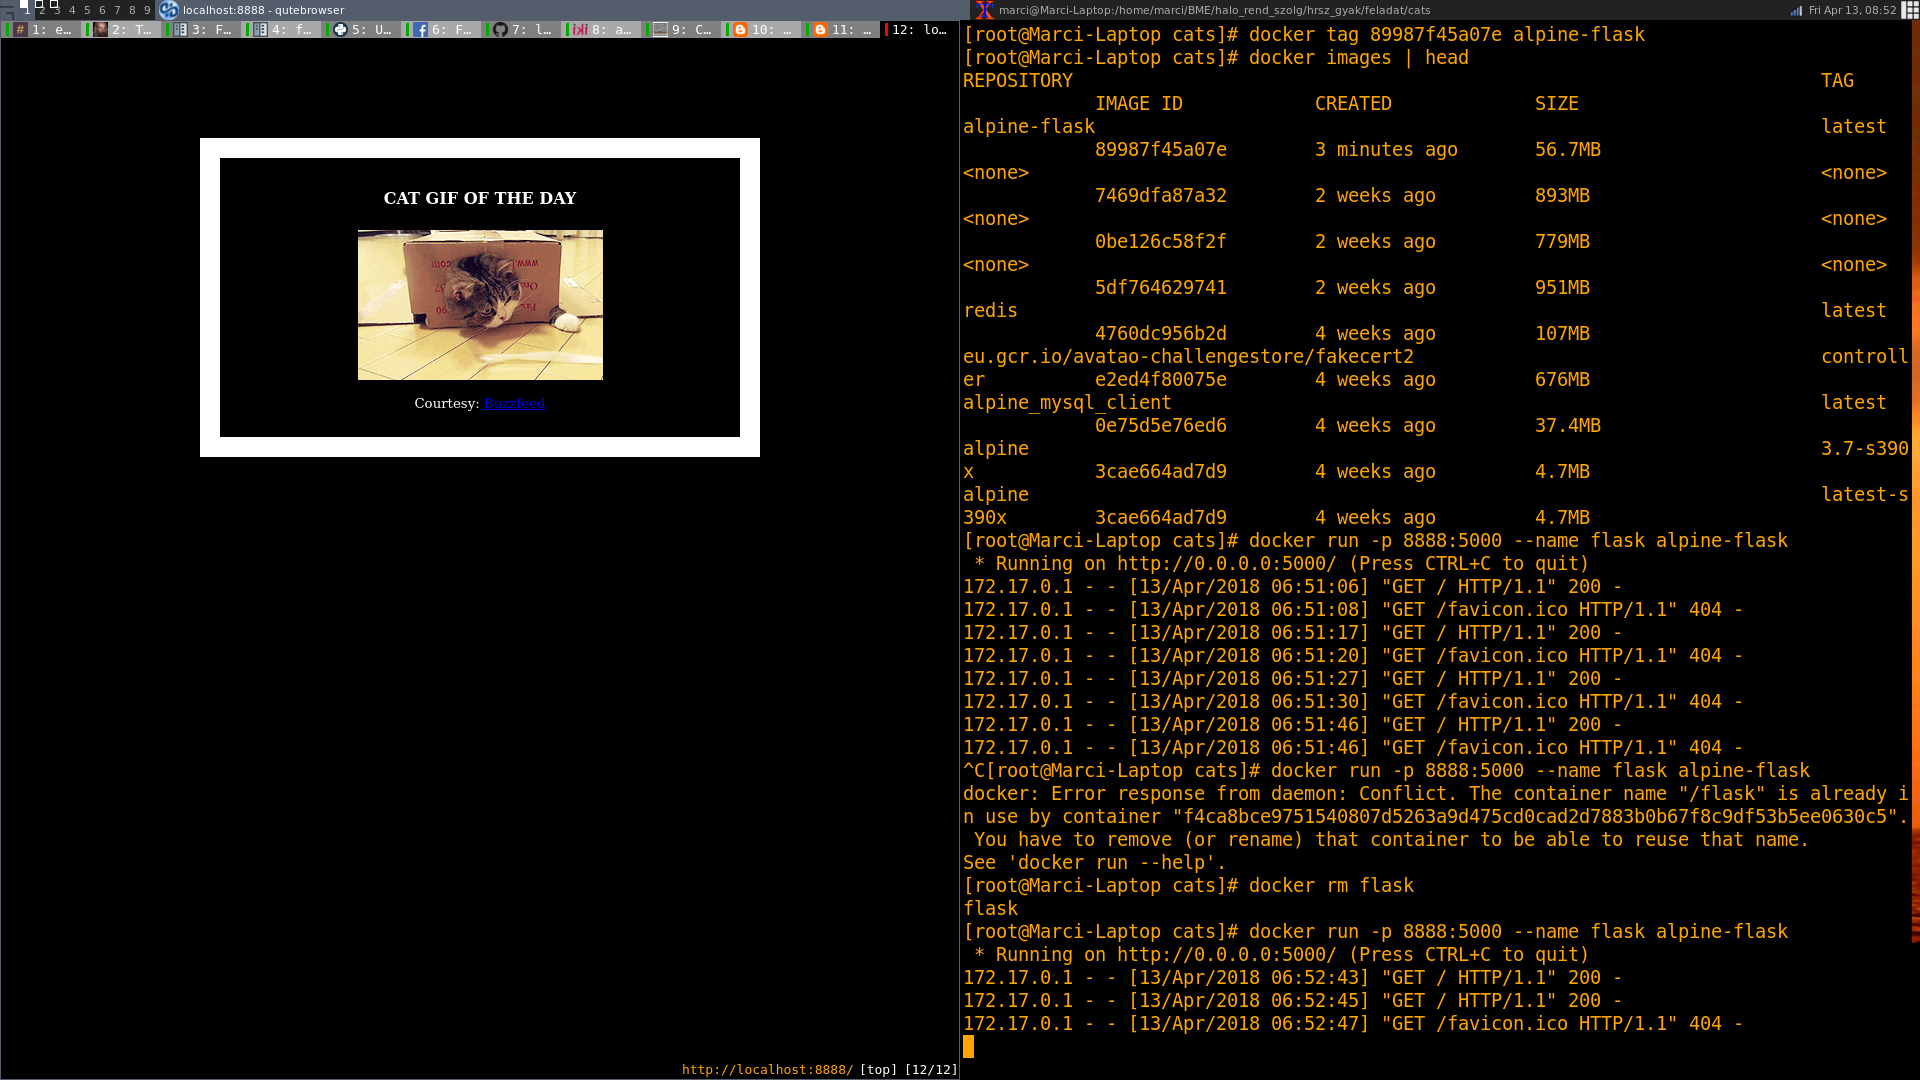
\includegraphics[width=0.9\linewidth]{cats}
	\caption{}
	\label{fig:cats}
\end{figure}

\section{Docker swarm}

A docker swarm lényege, hogy egy alkalmazást több containerben tudunl futtatni, így az erőforrásokat meg tudjuk osztani. A swarm tagjai containerek, amiknek két szerepük lehet: a manegerek irányítják a swarm működését, a workerek pedig elvégzik a feladatokat.

A swarm működtetéséhez először létrehoztunk két virtuális gépet, az egyikben a manager, a másikban a worker fog futni. Ezt az alábbi paranccsal tehetjük meg:

\texttt{docker-machine create --driver virtualbox myvm1}

\texttt{docker-machine create --driver virtualbox myvm2}

A \texttt{docker-machine ls} paranccsal listázhatjuk a futó virtuális gépeket, és az IP-címüket is megnézhetjük.

A swarmot az alábbi paranccsal hozhatjuk létre:

\texttt{docker-machine ssh myvm1 "docker swarm init --advertise-addr <myvm1 ip>"}

Ez a parancs a \texttt{myvm1} nevű gépben elindítja a swarmot. Ez a gép manager lesz. Létrehozáskor a swarm generál egy tokent, amire szükség van, amikor egy másik gép akar csatlakozni a swarmhoz. A swarmhoz workerként az alábbi paranccsal csatlakozhat a \texttt{myvm2} gép.

\texttt{docker-machine ssh myvm2 "docker swarm join --token <token> <ip>:2377"}

A docker swarm-ban service-eket futtathatunk. Egy service áll egy docker image-ből, valamint egyéb paraméterekből, például: containerek száma, CPU használati korlát, RAM használati korlát, port forwarding beállítások, stb. A mi példánkban egy korábban létrehozott, a docker hubra feltöltött image-et használtunk, amit 5 példányban futtattunk a swarmon.

A service-t a \texttt{docker-compose.yml} fájl írja le. Egy ilyen fájl például így nézhet ki:

\begin{figure}[H]
	\centering
	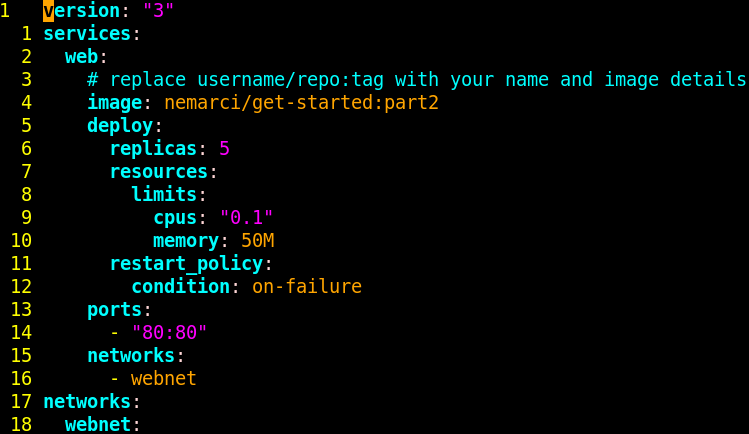
\includegraphics[width=0.7\linewidth]{service}
	\caption{}
	\label{fig:service}
\end{figure}

Ezt a service-t az alábbi paranccsal tudjuk futtatni a korábban létrehozott swarmon:

\texttt{docker-machine ssh myvm1 "docker stack deploy -c docker-compose.yml getstartedlab"}

Ezután a swarm elkezdi futtatni a fenti fájlban megadott service-t.

\end{document}
